\chapter{GAN}
Ein \glqq Generative Adversarial Net\grqq{} besteht aus zwei Teilstücken. Der erste Teil wird \glqq generative model $G$\grqq{}
genannt und generiert auf Basis eines originalen Datensets neue Datensamples. Der zweite Teil nennt sich \glqq discriminative model $D$\grqq{}
und schätzt die Wahrscheinlichkeit, ob ein solches Sample, welches $G$ generiert, aus dem originalen Datenset stammt. $D$
selbst hat als Output also eine reele Zahl. \cite{8253599}
In den Worten der Autoren ausgedrückt ist ein \Gls{GAN} ein Spiel zwischen Geldfälschern und Polizisten:
\itenquote{The generative model can be thought of as analogous to a team of counterfeiters,
trying to produce fake currency and use it without detection, while the discriminative model is
analogous to the police, trying to detect the counterfeit currency. Competition in this game drives
both teams to improve their methods until the counterfeits are indistiguishable from the genuine
articles} \cite{8253599}.
Anders ausgedrückt versucht $G$ immer besser zu werden, um $D$ möglichst zu überlisten. $D$ hingegen sieht sich einem immer
besser werdenden $G$ gegenüber gestellt und muss seine eigenen Schwachstellen ausbessern, um $G$ entgegenzuhalten. Eine Architektur, die
so aufgebaut ist, dass sie sich gegenseitig durch ein Konkurrenzverhalten immer weiter verbessert. Aus diesem Grund auch \glqq Generative \textbf{Adversarial} Net\grqq{} genannt.
\para
Im Endeffekt besteht das Ziel also darin, dass $D$ nicht mehr sagen kann, ob ein Sample von $G$ oder aus dem originalen Datenset stammt.
Somit sollte $D$ für alle Samples immer $\frac{1}{2}$ ausgeben. Dies bedeutet, dass ein Sample dieselbe Wahrscheinlichkeit
hat aus dem originalen Datenset oder aus dem generierten Set zu stammen und diese
beiden Datensets daher nicht mehr unterscheidbar sind.
Der Trainingsprozess für $G$ kann weiterhin als Maximierung der Fehlerwahrscheinlichkeit für $D$ angegeben werden. Dies entspricht also einem
Zwei-Spieler Minimax-Algorithmus\footnote{Für Erklärung, siehe Anhang \ref{anhang:minimax}}.\cite{8253599}
\para
Das generative Modell $G$ sowie das unterscheidende Modell $D$ bestehen jeweils aus zwei \Glspl{Multilayer perceptron}. Dies hat
den Vorteil, dass die Modelle mittels \Gls{Backpropagation} trainiert werden können \cite{8253599}. Eine kleine Einführung zu
neuronalen Netzen wird ebenso im Anhang unter \ref{anhang:neuronale_netze} gegeben.

\section{Funktionsweise}
Formell ausgedrückt besteht ein \Gls{GAN} aus zwei ableitbaren Funktionen $G(z;\theta_g)$ und $D(x,\theta_d)$, welche durch zwei \Glspl{Multilayer perceptron}
dargestellt werden. Dabei bilden jeweils $\theta_g$ sowie $\theta_d$ die Parameter der Netzwerke. Um die generierten Daten, welche der Wahrscheinlichkeitsverteilung $p_g$ folgen, über ein Sample $x$ aus
dem originalen Datenset, welche wiederum der Wahrscheinlichkeitsverteilung $p_{data}$ folgen, zu trainieren, wird eine vorgängige Verteilung $p_z(z)$ definiert. Diese bildet die
Wahrscheinlichkeitsverteilung der Noise-Samples. $G(z;\theta_g)$ bildet dabei das
Mapping zwischen diesen Noise-Daten und dem originalen Datenset.
Aus dem Noise wird also ein Sample erzeugt, welches möglichst mit den originalen Samples korreliert.
$D(x)$ wiederum gibt einen einzelnen Skalar aus, der die Wahrscheinlichkeit beschreibt, ob ein Sample $x$ eher aus dem originalen Datenset mit der Verteilung $p_{data}$
als aus dem generierten Datenset mit der Verteilung $p_g$ (beinhaltet alle Samples von $G$) stammt.
$D$ wird nun so trainiert, um die Wahrscheinlichkeit zu maximieren, das korrekte Label einem Input-Sample $x$ zu geben. Dabei gibt es zwei Labels:
\glqq Stammt aus original Datenset $D(x) = 1$\grqq{} und \glqq Stammt aus generiertem Datenset $D(x) = 0$\grqq{}. Simultan dazu wird $G$ trainiert, um die Funktion
$\log(1 - D(G(z)))$ zu minimieren\cite[p.~1]{8253599}. In Worten: $G(z)$ generiert ein Sample aus den Noise-Daten.
Davon wird die Wahrscheinlichkeit berechnet, ob dieses Sample aus dem originalen Datenset stammt. Geht dieser Wert gegen $1$, das heisst,
$D$ hat das Gefühl, dass das generierte Sample aus dem originalen Datenset stammt, so geht der Wert innerhalb des Logarithmus gegen 0 und damit gegen $-\infty$.
Dadurch wird also über diese Minimierung erzielt, dass $G$ möglichst Daten generiert, die $D$ nicht dem generierten Datenset sondern dem originalen Datenset selbst zuweist.
Die Autoren verweisen hier auf die Tatsache, dass die beiden neuronalen Netze $D$ und $G$ ein
Zwei-Spieler minimax-Spiel mit der folgenden Value-Funktion $V(D,G)$ spielen \cite[p.~2]{8253599}:
\begin{align}
    \min_{G} \max_{D} V(D, G) = E_{x\sim p_{data}(x)}[\log D(x)] + E_{z\sim p_z(z)}[\log(1 - D(G(z)))] \label{eq:1}
\end{align}
Nachfolgend werden einige Gedanken des Autors dazu aufgeführt.\\
\textbf{Fall 1 - Discriminator macht alles richtig}:
\begin{align}
    D(x) = 1, D(G(z)) = 0 \Rightarrow \ln(1) + \ln(1 - 0) = \ln(1) + \ln(1) = 0
\end{align}
\textbf{Fall 2 - Discriminator kann nicht mehr unterscheiden}:\\
\begin{align}
    D(x) = \frac{1}{2}, D(G(z)) = \frac{1}{2} \Rightarrow \ln(\frac{1}{2}) + \ln(1 - \frac{1}{2}) = \ln(\frac{1}{2}) + \ln(\frac{1}{2}) = -\ln(4) = -1.3862
\end{align}
Nach den Autoren bildet der Fall 2 das globale Optimum, welches eben nur erzielt werden kann, wenn der Discriminator nicht mehr zwischen
den beiden Datensets unterscheiden kann \cite[p.~4-5]{8253599}. Es gilt $p_{data} = p_{g}$. Wichtig zu beachten ist, dass sich die
beiden Verteilungen $p_{data}$ und $p_g$ über viele Trainingsschritte annähern und dadurch $D(x)$ für jedes Sample am Ende diese
$\frac{1}{2}$ ergeben sollte. Ist dies der Fall, so liegen die Verteilungen deckungsgleich übereinander und der Generator kann sich
nicht mehr verbessern. Sollte er sich trotzdem wieder von diesem Optimum entfernen, so wird der Fehler grösser und der Diskriminator
wird die generierten Bilder wiederum als nicht Originale erkennen. Um dies genauer zu erläutern, wird die Abbildung
\ref{fig:Verteilung} aus dem original Paper verwendet, wo ebendiese aufgezeigt werden.
\begin{figure}[h!]
    \begin{center}
        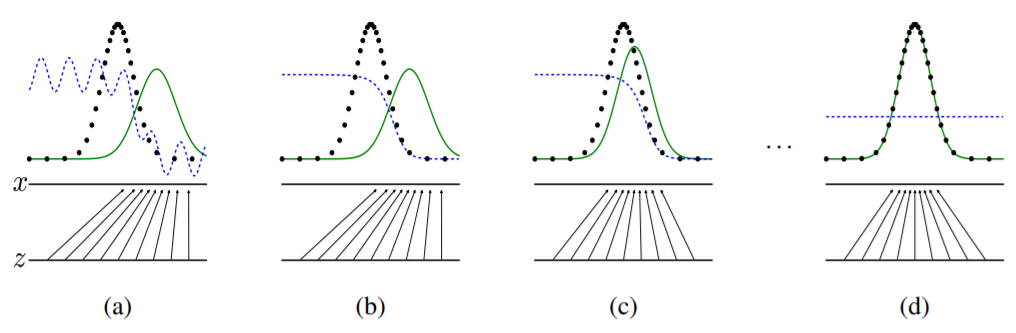
\includegraphics[width=0.8\textwidth]{../common/02_main/resources/06_verteilung.png}
    \end{center}
    \caption{Verteilung \cite{8253599}}
    \label{fig:Verteilung}
\end{figure}
In der Abbildung \ref{fig:Verteilung} wird aufgezeigt, wie ein Sample aus $Z$ auf ein Original in $X$ gemappt wird.
Dabei steht die gepunktete schwarze Linie für die Verteilung $p_{data}$ der originalen Samples, die grüne Linie für die Verteilung
$p_g$ der generierten Samples und die blaue Linie für den Diskriminator $D$.\\
a) Zu Beginn mappt der Generator die Samples aus $Z$ nicht gut auf die Originale in $X$, weswegen der Diskriminator gut
unterscheiden kann. Da die Verteilung der Originalen auf der linken Seite mächtiger ist, werden diese
als Originale eingestuft, die Samples auf der rechten Seite hingegen als Generierte. Im Laufe der Zeit wird
der Generator immer besser und seine Verteilung nähert sich der Originalen an, bis diese in
d) schliesslich deckungsgleich sind. Zu diesem Zeitpunkt kann der Diskriminator nicht mehr unterscheiden. Der Generator kann
nun nicht mehr besser werden, sollte er trotzdem seine Verteilung ändern, so kann der Diskriminator
wieder unterscheiden und wird wiederum wie bei a) verfahren. Offensichtlich geht man bei diesem Ansatz davon aus, dass der
Diskriminator $D$ für einen gegebenen Generator $G$ optimal trainiert ist, um die Verteilungen oder Samples unterscheiden
zu können.
\para
Bevor mit der Herleitung der GAN-Formel begonnen werden kann, müssen noch einige Worte über den Generator gesagt sein.
Bis jetzt drehte es sich vor allem um den Diskriminator, es stellt sich noch die Frage, wie denn der Generator lernt.
Nach \glqq Computerphile\grqq{} erhält $G$ Informationen von $D$.
$G$ kennt also die Schwächen von $D$ und kann diese besser ausnützen \cite{youtube:gan}. Im ersten Teil der Arbeit wurde
bereits ein wenig darauf eingegangen. Dieses Wissen wird nun über einen zusätzlichen Artikel noch ein wenig erweitert, um
auch den Praxisbezug herzustellen. Es handelt sich dabei um einen Artikel, der sich einem Beispiel in Tensorflow widmet \cite{tensorflow:1:gan}.
Dieser Artikel wird auch den Anstoss zur Herleitung von $V(D,G)$, also der Formel \ref{eq:1}, geben.
In diesem Artikel wird eine Loss-Funktion\footnote{Die Loss-Function bildet die Bewertung eines neuronalen Netzes. Sie gleicht eine Menge von Wahrscheinlichkeiten eines
Ereignisses mit einer anderen ab und soll $0$ ergeben, wenn die Mengen identisch sind.\cite{wiki:lossFunction}}
sowohl für den Generator, wie auch den Discriminator angegeben. Die Loss-Funktionen werden im nachfolgenden einzeln besprochen, zuerst wird sich dem Generator gewidmet.
\begin{lstlisting}
    def generator_loss(fake_output):
        return cross_entropy(tf.ones_like(fake_output), fake_output)
\end{lstlisting}
Die Loss-Funktion nach \cite{tensorflow:1:gan} für den Generator besteht also im Wesentlichen aus einer Kreuzentropie\footnote{Beschreibung in
Anhang \ref{anhang:kreuzentropie}} zwischen der Wahrscheinlichkeit des Diskriminators für die generierten Samples \glqq fake\textunderscore output\grqq{}
sowie der Wahrheit (alle Wahrscheinlichkeiten sind in dem Fall $1$). Dies bedeutet, der Fehler für den Generator ist $0$, wenn der Diskriminator
alle generierten Samples als Sample aus dem originalen Datenset anerkennt. Diese Interpretation ist also in Theorie und Praxis soweit dieselbe.\\
Für den Diskriminator ist die Sache ein wenig komplizierter \cite{tensorflow:1:gan}.
\begin{lstlisting}
    def discriminator_loss(real_output, fake_output):
        real_loss = cross_entropy(tf.ones_like(real_output), real_output)
        fake_loss = cross_entropy(tf.zeros_like(fake_output), fake_output)
        total_loss = real_loss + fake_loss
        return total_loss
\end{lstlisting}
An dieser Stelle werden nun die einzelnen Zeilen der Gleichung \ref{eq:1} zugewiesen. Dazu muss bekannt sein, dass der
Diskriminator ein binäres Problem beschreibt, das heisst, er sollte eigentlich nur die Werte $0$ und $1$ annehmen.
Weiterhin scheint die Gleichung \ref{eq:1} der Kreuzentropie entnommen zu sein. Diese
kann für einen binären Klassifizierer wie in Formel \ref{eq:7} geschrieben werden \cite{stackoverflow:1:crossEntropy}
\footnote{Wieso die Kreuzentropie geeignet ist und wie die Herleitung aussieht, siehe Anhang \ref{anhang:binary:kreuzentropie}}.
\begin{align}
    H(P,Q) = - \sum_{x \in X} (P(x) \cdot log(Q(x)) + (1 - P(x)) \cdot log(1 - Q(x))) \label{eq:7}
\end{align}
Die erste Zeile der \glqq discriminator\textunderscore loss\grqq{} Funktion berechnet die Kreuzentropie zwischen den Wahrscheinlichkeiten der originalen Samples
sowie der erwarteten Wahrscheinlichkeiten von $D$ für die originalen Samples. Für den Diskriminator entspricht $P(x) = 1$ für alle Wahrscheinlichkeiten,
wobei $Q(x) = D(x)$ gilt und das Sample $x$ aus dem originalen Datenset stammt. Eingesetzt in Formel \ref{eq:7} ergibt dies \ref{eq:8}.
\begin{align}
    H(P,D) = - \sum_{x \sim p_{data}} (P(x) \cdot log(D(x)) + (1 - P(x)) \cdot log(1 - D(x))) \label{eq:8}\\
    H(1,D) = - \sum_{x \sim p_{data}} log(D(x)) \label{eq:11}
\end{align}
Die darauffolgende Zeile der Funktion \glqq discriminator\textunderscore loss\grqq{} wird dem zweiten Summand der Gleichung \ref{eq:1} zugewiesen.
In diesem Fall ist $P(x) = 0$ für alle erwarteten Wahrscheinlichkeiten (das generierte Sample gehört nicht zum
originalen Datenset), $Q(x) = D(x)$ und $x$ stammt aus dem generierten Datenset.
\begin{align}
    H(P,D) = - \sum_{x \sim p_{g}} (P(x) \cdot log(D(x)) + (1 - P(x)) \cdot log(1 - D(x)))\\
    H(0,D) = - \sum_{x \sim p_{g}} log(1 - D(x)) \label{eq:9}
\end{align}
Wenn nun in Betracht gezogen wird, dass $z$ der Noise-Verteilung $p_z$ folgt und $x = G(z)$ gilt,
dann kann die Formel \ref{eq:9} so umgeschrieben werden, dass sie mit der Formel \ref{eq:1} korreliert.
\begin{align}
    H(0,D(G)) = - \sum_{z \sim p_{z}} log(1 - D(G(z))) \label{eq:10}
\end{align}
Zusammenaddiert ergeben die Formeln \ref{eq:11} und \ref{eq:10} fast den Loss-Wert der Formel \ref{eq:1} und damit auch die Minimax-Value-Funktion,
welche nach den Formeln \ref{eq:11} und \ref{eq:10} eigentlich von $D$ minimiert werden will.
\begin{align}
    \widetilde{V(D,G)} = - \sum_{x \sim p_{data}} log(D(x)) - \sum_{z \sim p_{z}} log(1 - D(G(z)))
\end{align}
Es muss nun noch berücksichtigt werden, dass effektiv der Erwartungswert der Summanden von $\widetilde{V(D,G)}$ relevant ist. Daher
wird $\widetilde{V(D,G)}$ um den Zusatz des arithmetischen Mittels\footnote{Vom Erwartungswert zum arithmetischen Mittel, siehe Anhang \ref{anhang:erwartungswert}} erweitert und im gleichen Zuge wird ebenfalls noch
$-1$ ausgeklammert. Es resultiert die Formel \ref{eq:13} wenn genau $m$ Samples ausgewählt werden.
\begin{align}
    \widetilde{V(D,G)} = - \frac{1}{m} \cdot (\sum_{x \sim p_{data}} log(D(x)) + \sum_{z \sim p_{z}} log(1 - D(G(z))))\label{eq:13}
\end{align}
Formel \ref{eq:12} erklärt nun den Zusammenhang zwischen der über die Kreuzentropie hergeleiteten Formel wie auch der Value-Function aus Formel \ref{eq:1}.
\begin{align}
    -\widetilde{V(D,G)} = V(D,G)\label{eq:12}
\end{align}
Für den Minimax-Algorithmus wird also die Richtung der Optimierung umgedreht, um nach $G$ zu minimieren.

\newpage
\section{Lernprozess}
Der Algorithmus sieht vor, dass zuerst der Diskriminator $D$ trainiert wird. Dazu wird $k$-mal ein Minibatch aus
den Noise-Samples wie auch aus den originalen Samples geladen. Der Diskriminator wird dann anhand der Formel \ref{eq:1}
aktualisiert.
Nach diesen $k$-Schritten wird wiederum ein Minibatch von Noise-Samples geladen und der Generator damit trainiert.
Dieser Ablauf ist aus dem Algorithmus \ref{alg:1} ersichtlich, welcher von den Autoren des Papers beschrieben wird \cite{8253599}.

\begin{algorithm}[H]
    \For{number of epochs}{
        \For{k steps}{
            Sample minibatch of $m$ noise samples $\{z^{(1)}, \cdots, z^{(m)}\}$ from noise prior $p_{g}(z)$\\
            Sample minibatch of $m$ originals ${x^{(1)}, \cdots, x^{(m)}}$ from original data generating distribution $p_{data}(x)$\\
            Update the discriminator by ascending its stochastic gradient:\\
            $\nabla_{\theta_d} \frac{1}{m}\sum_{i=1}^{m}[\log D(x^{(i)}) + \log(1 - D(G(z^{(i)})))]$
        }
        Sample minibatch of $m$ noise samples $\{z^{(1)}, \cdots, z^{(m)}\}$ from noise prior $p_{g}(z)$\\
        Update the generator by descending its stochastic gradient:\\
        $\nabla_{\theta_g} \frac{1}{m}\sum_{i=1}^{m}[\log(1 - D(G(z^{(i)})))]$
    }
    \caption{Algorithmus}
    \label{alg:1}
\end{algorithm}

\section{Noise zu Sample}
Die Problematik der Bildgenerierung an sich wurde zu Beginn ein wenig angedeutet. Dies soll nun vertieft
werden. Nach \glqq Computerphile \grqq{} lernt ein Neuronales Netz die Klassifikation auf ein Label. Das heisst, es gibt
jeweils genau eine richtige Lösung \cite[~t 4:00]{youtube:gan}. Die Problematik besteht nun darin, dass es in diesem Fall eine
unendliche Menge an korrekten Lösungen gibt. Es kann also eine Lösung bei einem \Gls{KNN} angefragt werden, die erhaltene
Lösung muss dann aber mit einer Art \glqq Zufälligkeit\grqq{} verändert, respektive korrigiert werden.
\para
Wie Eingangs erwähnt, bildet $G$ ein Mapper von Noise-Samples $z$ nach Samples $x \sim p_{data}$. Weiterhin ist nach
dem Beispiel in Tensorflow das neuronale Netz von $G$ als \Gls{CNN} definiert. Wahrscheinlich entspricht die Input-Dimension des
Bilds der Output-Dimension \cite{tensorflow:1:gan}. Damit ist die Antwort auf die Frage bereits vornweg genommen.
Die Frage selbst lautet, wie der Generator Bilder erzeugt. Um dies trotzdem ein wenig genauer zu erläutern wird zu Beginn
ein neuronales Netz angenommen, das lediglich ein einzelnes Neuron in der Input-Schicht hat. Der Definitionsbereich dieses Neurons sei
weiterhin auf $0$ und $1$ beschränkt, ist also binär. Dementsprechend kann der Generator logischerweise genau zwei Bilder
generieren, da es sich um einen deterministischen Algorithmus handelt, welcher keinerlei Zufälligkeit zulässt.
\para
Irgendwoher muss diese Zufälligkeit dem Generator zugeführt werden. Dies geschieht nun eben bei diesem Input-Layer.
Bei einem klassischen \Gls{KNN} kann es also nicht einfach nur ein Neuron geben. Es gibt eine ganze Menge und der Wert
der einzelnen Inputs kann zwischen bestimmten Intervallen liegen. Weiterhin werden alle Werte zufällig bestimmt,
was einem Rauschen gleichkommt, wie in Abbildung \ref{fig:Input-Noise} ersichtlich ist.
\begin{figure}[h!]
    \begin{center}
        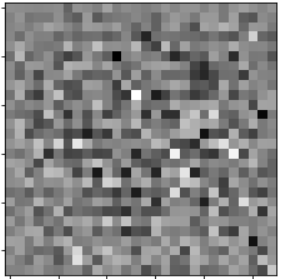
\includegraphics[width=0.5\textwidth]{../common/02_main/resources/05_noise.png}
    \end{center}
    \caption{Input-Noise \cite{tensorflow:1:gan}}
    \label{fig:Input-Noise}
\end{figure}
\para
Was genau bedeutet nun dieses Rauschen? Nach \glqq Computerphile\grqq{} kann dieses Rauschen einem Punkt in einem
mehrdimensionalen Raum gleichgesetzt werden \cite[~t 16:45]{youtube:gan}. Wird dieser Punkt leicht angepasst, dann
wird der Generator daraus ein leicht anderes Sample erzeugen, das einem Sample aus dem originalen Datenset entspricht.
Eine Richtung in diesem mehrdimensionalen Raum kann ebenfalls bestimmten Eigenschaften zugewiesen werden. Wird der Punkt
z.B. in nur eine Richtung verschoben, so wird ein Objekt auf dem Output-Sample leicht grösser. Eine
Richtung in diesem Raum würde also der Grösse entsprechen \cite[~t 17:35]{youtube:gan}.

\section{Vor- und Nachteile}
Ein grosser Nachteil ist, dass $D$ und $G$ während dem Training synchronisiert werden müssen, $G$ kann also nicht
häufig trainiert werden ohne auch $D$ zu aktualisieren. Ansonsten könnte das \glqq Helvetica Szenario\grqq{} eintreten,
wo $G$ sehr viele Samples aus dem Noise-Raum der Verteiltung $p_z$ auf dasselbe Sample im originalen Raum abbildet \cite{8253599}.
Es muss weiterhin beachtet werden, dass die beiden Kontrahenten etwa gleich stark sind, ansonsten hat der anderer keine
Chance sich zu verbessern.
\para
Vorteile betreffen das Lernen an sich. So muss nur \Gls{Backpropagation} eingesetzt werden, um Gradienten zu finden.
Es kann auch gut sein, dass statistische Vorteile erzielt werden durch die Tatsache, dass der Generator $G$ nicht direkt
mit Samples aus den Testdaten sondern nur mit Informationen von $D$ aktualisiert wird. Die Autoren verweisen hier auf
den Fakt, dass Komponenten der Testdaten nicht direkt die Parameter des Generators beeinflussen \cite{8253599}.